\section{Bombas Térmiacs}

Una bomba térmica (BT), es un dispositivo el cual tiene la capacidad de
recibir trabajo externo, y operar en un sistema con dos reservorios,
uno a temperatura $T_A$ y otro a temperatura $T_B$ con $T_B < T_A$. La BT
absorve una cantidad de calor $Q_B'$ del reservorio a temperatura baja, y cede
una cantidad de calor $Q_A'$ al reservorio a temperatura alta.

\begin{center}
  \begin{tikzpicture}
    \draw[domain=0:360, samples=500] plot ({3*cos(\x)},{sin(\x)+4});
      \node at (0,4) {$T_A$};
    \draw[domain=0:360, samples=500] plot ({cos(\x)},{sin(\x)});
      \node at (0,0) {BT};
    \draw[domain=0:360, samples=500] plot ({3*cos(\x)},{sin(\x)-4});
      \node at (0,-4) {$T_B$};

    \draw[stealth-] ({3*cos(deg(-0.5*pi))},{sin(deg(-0.5*pi))+4}) 
    -- (-0.2, 1.8) -- (0.2,2.2) -- ({cos(deg(0.5*pi))},{sin(deg(0.5*pi))});
      \node at (0.6,2) {$Q_A'$};
    \draw[stealth-]  ({cos(deg(-0.5*pi))},{sin(deg(-0.5*pi))})
    -- (-0.2, -2.2) -- (0.2,-1.8) -- ({3*cos(deg(0.5*pi))},{sin(deg(0.5*pi))-4});
      \node at (0.6,-2) {$Q_B'$};
    \draw[stealth-] (-1,0) -- (-2,0); 
      \node at (-2.2, 0) {$T_r$};
  \end{tikzpicture}
\end{center}

De igual forma a las máquinas térmicas, la BT requiere una sustancia de
trabajo, la cual también opera en un ciclo, por lo que, considerando este
ciclo, los cambios de energía deben ser nulos, pues se retorna a la
temperatura con la que comenzó.

\begin{longderivation}
  \res{ \Updelta U = Q + T_r }\\
\why{ Se finaliza en el mismo estado en el que se inició }\\
  \res{ Q = -T_r }
\end{longderivation}

La transferencia neta de calor debe ser la energía que recibe, menos la
energía que cede, así:

\[Q = Q_B' - Q_A' \quad\land\quad T_r = Q_A' - Q_B'\]

Igualmente, se puede medir la eficiencia de una BT, esto sería la razón
entre la energía entregada y la energía recibida.

Debido a como funcionan, este cociente puede llegar a ser mayor que $1$,
por lo que no coincide del todo con la definición de eficiencia. Por esta
razón se le da el nombre de coeficiente de operación, en estos casos.

Las BT, tienen dos modalidades:
\begin{enumerate}
  \item Refrigerador:

        En esta modalidad, se busca enfriar un ambiente interno, por lo que
        los reservorios serían respectivamente, en el ejemplo de una nevera:

        \begin{center}
          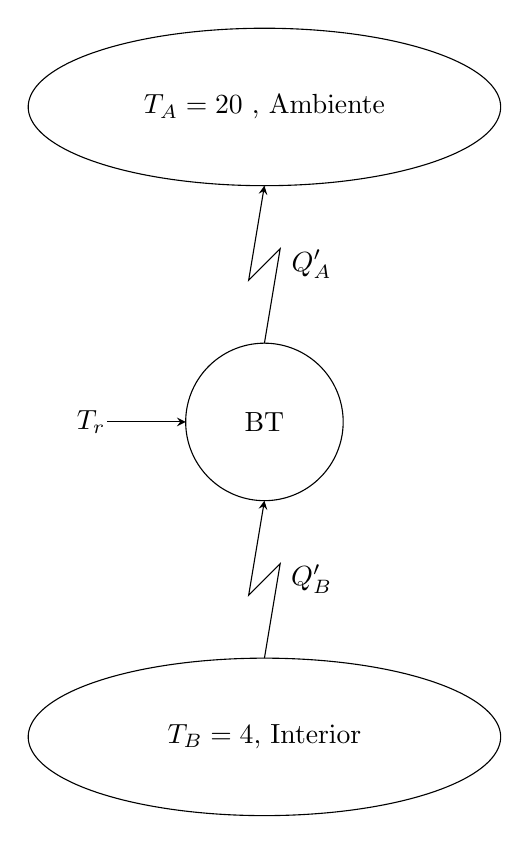
\begin{tikzpicture}
            \draw[domain=0:360, samples=500] plot ({3*cos(\x)},{sin(\x)+4});
              \node at (0,4) {$T_A=\qty{20}{\degreeCelsius}$ , Ambiente};
            \draw[domain=0:360, samples=500] plot ({cos(\x)},{sin(\x)});
              \node at (0,0) {BT};
            \draw[domain=0:360, samples=500] plot ({3*cos(\x)},{sin(\x)-4});
              \node at (0,-4) {$T_B=\qty{4}{\degreeCelsius}$, Interior};
        
            \draw[stealth-] ({3*cos(deg(-0.5*pi))},{sin(deg(-0.5*pi))+4}) 
            -- (-0.2, 1.8) -- (0.2,2.2) -- ({cos(deg(0.5*pi))},{sin(deg(0.5*pi))});
              \node at (0.6,2) {$Q_A'$};
            \draw[stealth-]  ({cos(deg(-0.5*pi))},{sin(deg(-0.5*pi))})
            -- (-0.2, -2.2) -- (0.2,-1.8) -- ({3*cos(deg(0.5*pi))},{sin(deg(0.5*pi))-4});
              \node at (0.6,-2) {$Q_B'$};
            \draw[stealth-] (-1,0) -- (-2,0); 
              \node at (-2.2, 0) {$T_r$};
          \end{tikzpicture}
        \end{center}

        En este ejemplo, la sustancia de trabajo viene a ser un líquido,
        el cual tenga su temperatura de fusión bastante más baja que la
        tamperatura deseada. Suponga \qty{-30}{\degreeCelsius}. El
        trabajo es generado por la compresión y descompresión de este
        líquido, haciendo que pase de una temperatura a otra. El ciclo
        en el que se mantiene es:
        \begin{enumerate}
          \item El líquido va a una temperatura de \qty{-5}{\degreeCelsius}.
          \item Al pasar por el serervorio con temperatura interior, pasa a
                \qty{4}{\degreeCelsius}.
          \item Vuelve a la BT, de la cual sale al reservorio exterior a
                temperatura \qty{30}{\degreeCelsius}.
          \item Al pasar por el ambiente, cede calor y vuelve con temperatura
                \qty{20}{\degreeCelsius}. En la BT, vuelve a su temperatura
                inicial y repite el ciclo
        \end{enumerate}
  \item Calentador:
        
        En esta modalidad, el proceso realmente es el mismo, sin embargo, ahora
        es el exterior el que está a menor temperatura, y el interior está a mayor.
        La diferencia radica únicamente en la perspectiva de cual de los dos entornos
        se quiere mantener a una temperatura no natural. Desde un punto de vista donde
        el entorno está a \qty{4}{\degreeCelsius} y un entorno interor (un cuarto por
        ejemplo) se quiere mantener a \qty{20}{\degreeCelsius}, se realiza el mismo
        proceso, solo que visto desde el otro punto de vista.
\end{enumerate}

La segunda ley de la termodinámica también se puede expresar en términos
de las BT:

No es posible construir o encontrar una BT la cual, sin recibir un trabajo
externo, sea capáz de recibir una energía $Q_B$ de un reservorio a
temperatura baja $T_B$, y entregar una energía $Q_A$ a otro reservorio
a temperatura alta $T_A$.

\[T_r > 0\]